\chapter{Laboratorium II}\label{ch:lab2}

\section{Wybrany sprzęt}\label{sec:lab2-hw}

System modułów \emph{Grove} jest~wykorzystany w~dwóch laboratoriach, w~związku z~czym jego~opis znajduje~się w~sekcji
przodującej (\ref{subsec:grove}).
W~tym laboratorium zostały użyte dwa~urządzenia współpracujące z~\emph{Grove Base HAT}.

Głównym komponentem jest~czujnik odległości wykorzystujący fale ultradźwiękowe.

Do~wyświetlenia wyników pomiaru wybrany został wyświetlacz LCD $2\,\times\,16$ komórek o wielkości komórki $8x5$.

\section{Dodatkowe oprogramowanie}\label{sec:lab2-sw}

\emph{Seeed-grove.py} to oficjalna biblioteka zestawu Grove, niestety niedostępna przy~wykorzystaniu standardowego
repozytorium bibliotek języka \emph{Python}.
Kod biblioteki można zobaczyć na~platformie \emph{GitHub}\thinspace\cite{grovelib}.
Dzięki~temu możliwa nadal~jest stosunkowo prosta instalacja (rys.~\ref{fig:seeed}).

\begin{figure}[H]
  \lstinputlisting[language=sh,label={lst:seeed}]{media/seeed.sh}
  \caption{Instalacja biblioteki \emph{grove} z~platformy \emph{GitHub}}
  \label{fig:seeed}
\end{figure}

\section{Rozwiązanie}\label{sec:lab2-sol}

Rysunek~\ref{fig:distancelab} to~fragment instrukcji przestawiający dwa z~zadań składających~się na~końcowy program
mierzący odległość do~obiektu przy~wykorzystaniu sensora ultradźwiękowego.

\begin{figure}[H]
  \centering
  \includegraphics[width=0.9\linewidth]{media/distance_lab}
  \caption{Fragment instrukcji ``Odległość''}
  \label{fig:distancelab}
\end{figure}

Rysunek~\ref{fig:distance} przedstawia rozwiązanie zadania.
W~tym przypadku podana odległość jest~do~telefonu, którym~utworzone zostało to~zdjęcie, a~wyświetlacz jest~w~trakcie
zmiany wyświetlanej wartości.

\begin{figure}[H]
  \centering
  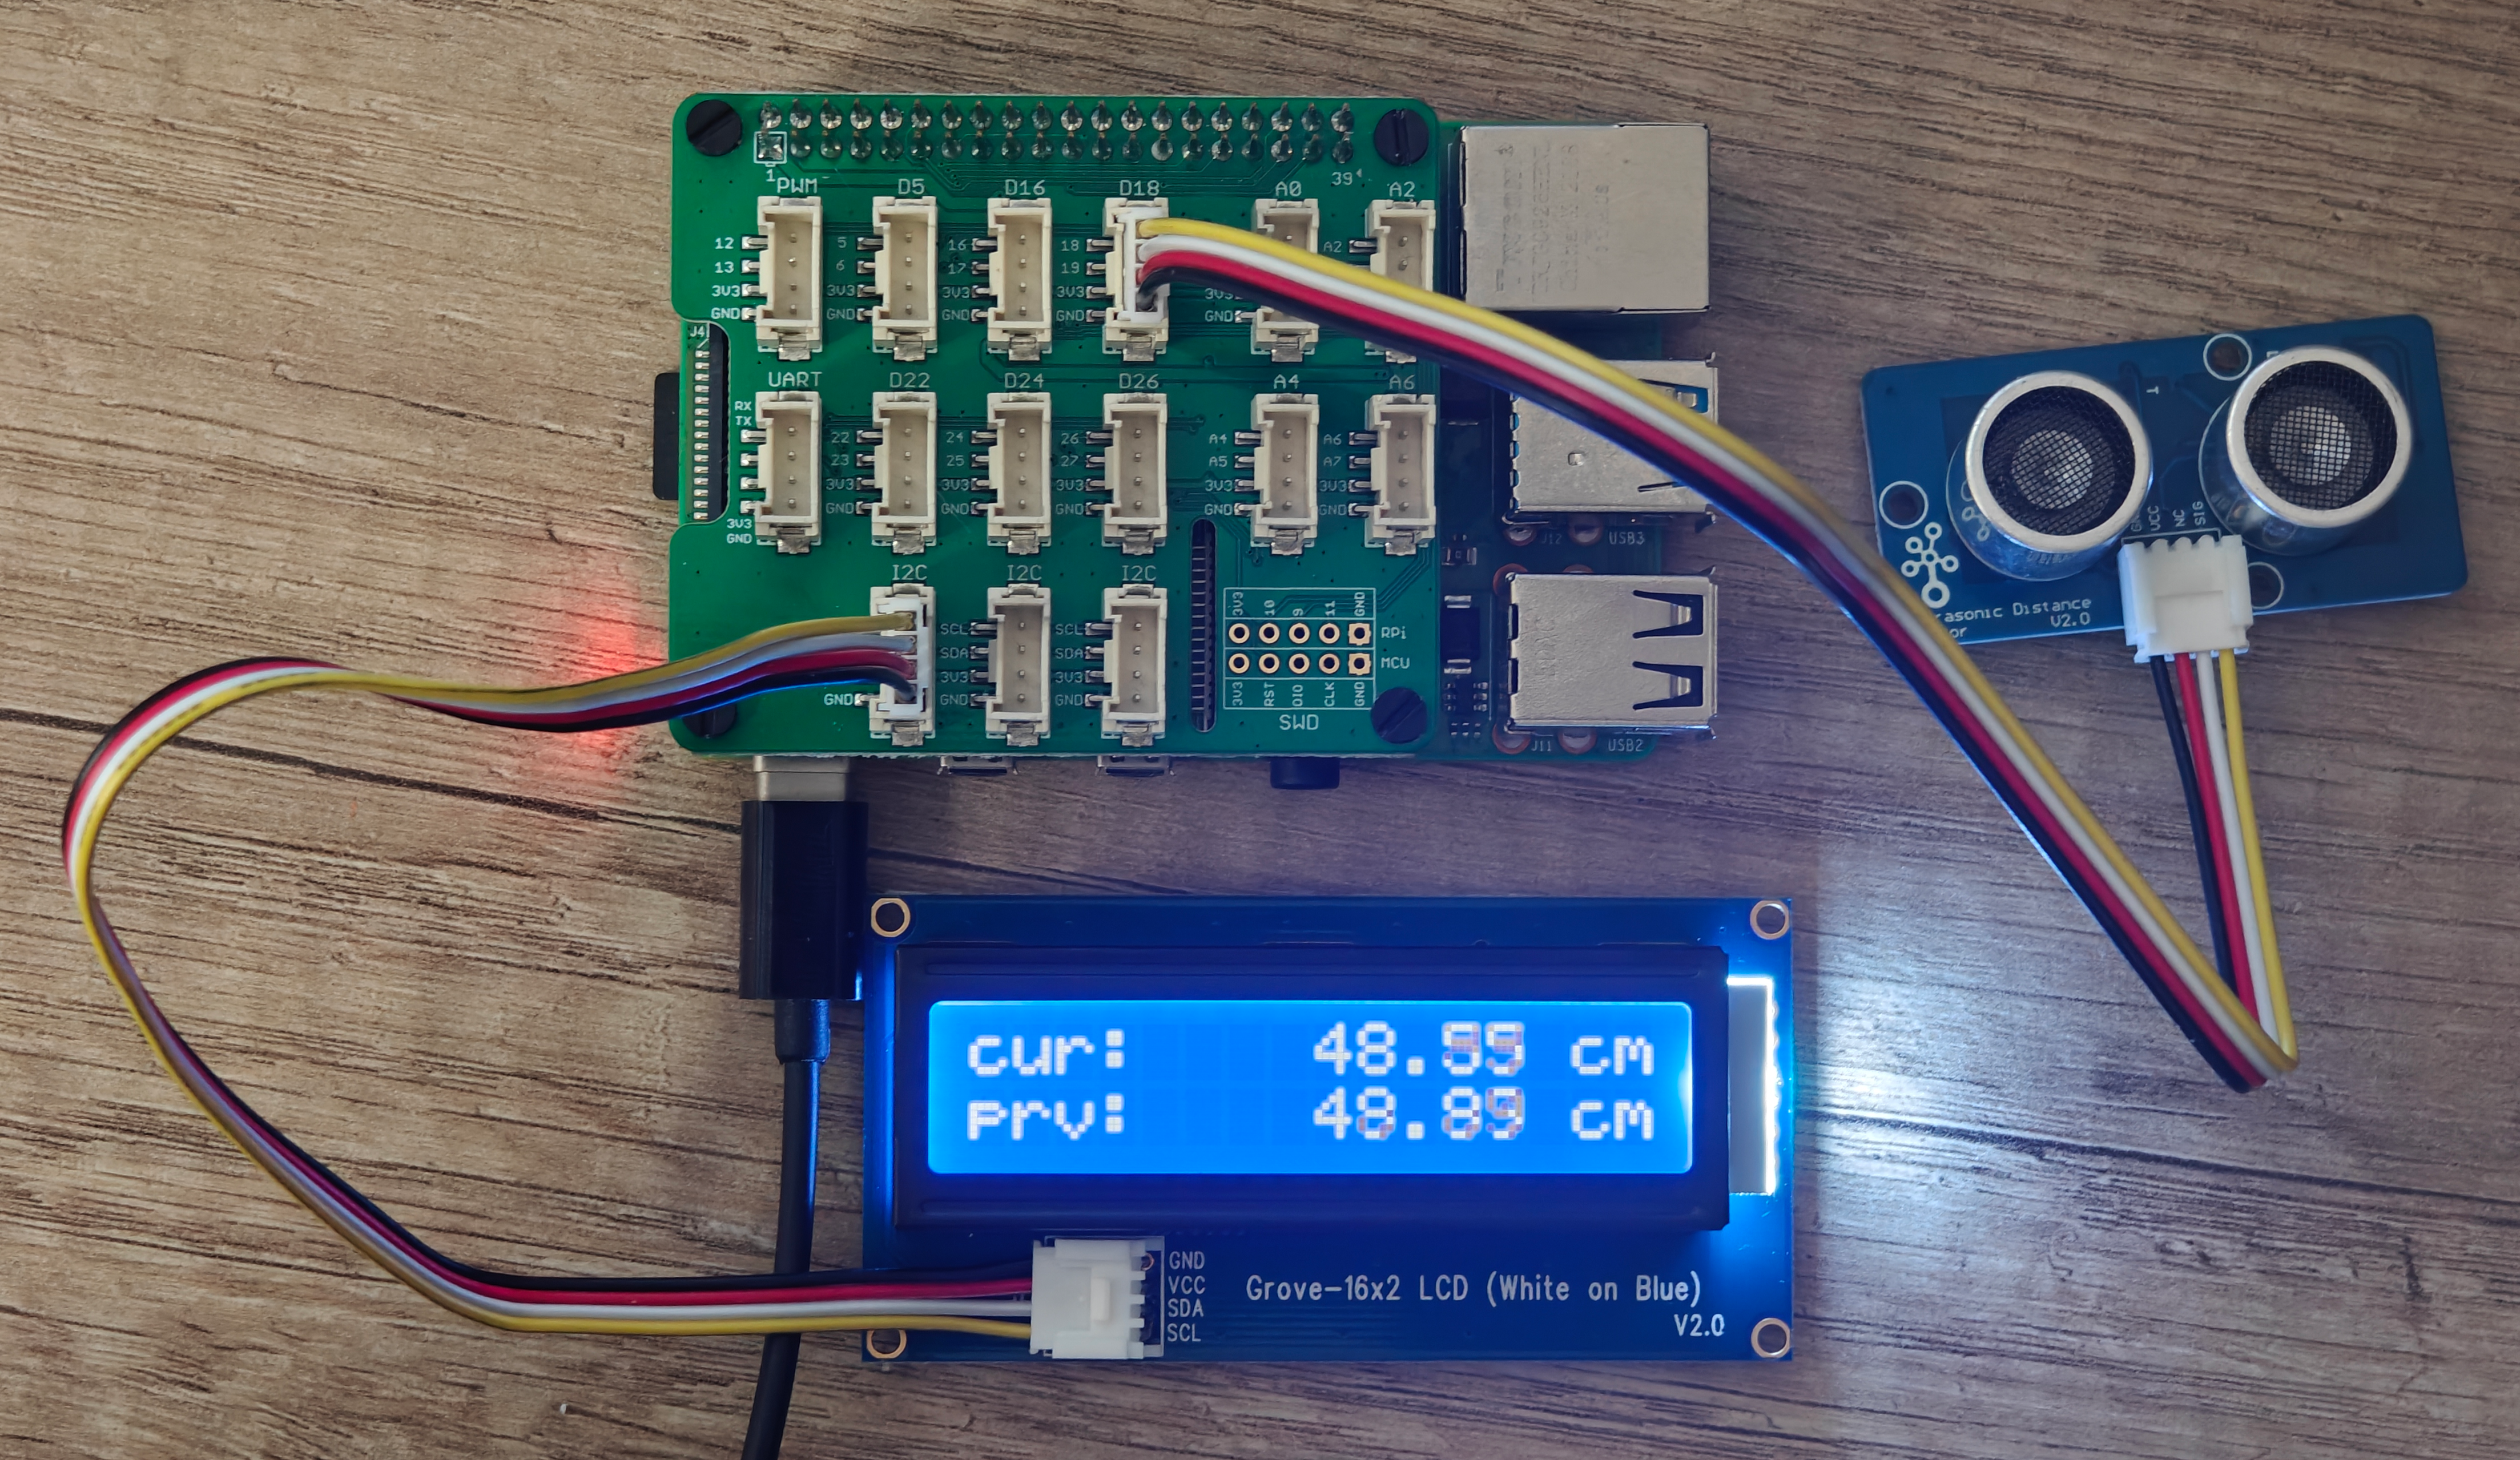
\includegraphics[width=0.6\linewidth]{media/distance}
  \caption{Uruchomiony program drugiego laboratorium}
  \label{fig:distance}
\end{figure}
